\documentclass[10pt,a4paper]{article}
\usepackage[utf8x]{inputenc}
\usepackage[T1]{fontenc}
%\usepackage{stringenc} % for grffile
\usepackage{ucs}
\usepackage{amsthm} %numéroter les questions
\usepackage[english]{babel}
\usepackage{datetime}
\usepackage{xspace} % typographie IN
\usepackage{hyperref}% hyperliens
\usepackage[all]{hypcap} %lien pointe en haut des figures
\usepackage[english]{varioref} %voir x p y
\usepackage{fancyhdr}% en têtes
%\input cyracc.def
\usepackage[]{graphicx} %include pictures
%\usepackage[encoding,inputencoding=utf8,filenameencoding=utf8]{grffile}
%\usepackage[extendedchars,inputencoding=latin1,filenameencoding=latin1]{grffile}
\usepackage[siunitx ]{circuitikz}
\usepackage{gnuplottex}
\usepackage{ifthen}
\graphicspath{{./figures/}}
%\usepackage{array}
\usepackage{amsmath}
\usepackage[]{xcolor}
\usepackage{tikz}
\usepackage{tikz-timing}
\usetikzlibrary{scopes}
\usetikzlibrary{backgrounds}
\usepackage{listings}
\usepackage{enumitem}
\usepackage[top=1 in, bottom=1 in, left=1.3 in, right=1 in]{geometry} % Yeah, that's bad to play with margins
\usepackage[]{pdfpages}
\usepackage{pdflscape}
\usepackage[]{attachfile}
%\usepackage{colortbl}
%\usepackage{multirow}
\usepackage{booktabs}
\usepackage{makecell}
\usepackage[ ]{subfig}
%\usepackage{rotating}
\usepackage{upgreek}
\usepackage[normalem]{ulem}

\newdateformat{mydate}{2017--2018}%hack pour remplacer \THEYEAR

%cyr
%\newcommand\textcyr[1]{{\fontencoding{OT2}\fontfamily{wncyr}\selectfont #1}}
\renewcommand{\marginpar}[1]{} %surcharge pour /marginpar

\newboolean{corrige}
%\setboolean{corrige}{true}%corrigé
\setboolean{corrige}{false}% pas de corrigé

\newboolean{annexes}
%\setboolean{annexes}{true}%annexes
\setboolean{annexes}{false}% pas de annexes

\newboolean{mos}
%\setboolean{mos}{true}%annexes
\setboolean{mos}{false}% pas de annexes

\usepackage{aeguill} %guillemets

%% fancy header & foot
\pagestyle{fancy}
\lhead{[ELEC-H-410] Real-Time systems Lab n° 1: \uCOSII}
\rhead{\mydate\today\\ page \thepage}
\chead{\ifthenelse{\boolean{corrige}}{Corrigé}{}}
\cfoot{}
%%

\pdfinfo{
/Author (Yannick Allard - Raoul Sommeillier, ULB -- BEAMS)
/Title (Lab n° 1 ELEC-H-410, uCOS-II)
/ModDate (D:\pdfdate)
}

\hypersetup{
pdftitle={Lab n° 1 [ELEC-H-410] Real-Time systems},
pdfauthor={Yannick Allard - Raoul Sommeillier, ©2014-17 ULB - BEAMS  },
pdfsubject={uCOS-II}
}

\theoremstyle{definition}% questions pas en italique
\newtheorem{E}{\color{blue}Exercise}[] % numéroter les questions [section] ou non []

\newcommand{\reponse}[1]{% pour intégrer une réponse : \reponse{texte} : sera inclus si \boolean{corrige}
	\ifthenelse {\boolean{corrige}} {\paragraph{Réponse :} #1} {}
 }

\newcommand{\addcontentslinenono}[4]{\addtocontents{#1}{\protect\contentsline{#2}{#3}{#4}{}}}

\newcommand{\on}[1]{\operatorname{#1}}

\newcommand{\reg}[1]{\texttt{reg#1}}

\newcommand{\uCOSII}{$\upmu$C/OS-II}

\newcommand{\kw}[1]{\texttt{#1}}

\setlength{\parskip}{1ex plus .5ex minus .5ex} % espacement entre paragraphes
\setlength{\parindent}{0 ex plus 0ex minus 0 ex} % retrait en début de §

\def\labelitemi{--}
\setlist{parsep=0pt,itemsep=0pt,style=standard,leftmargin=\parindent, align=left} % pas d'espace prohibitif entre les items
\setlist{nolistsep}

\newcolumntype{C}[1]{>{\centering\let\newline\\\arraybackslash\hspace{0pt}}m{#1}}

%\setlength{\tabcolsep}{0pt} %no extra space in cells to keep constant tabular width

\date{\vspace{-1cm}\mydate\today}
\title{\vspace{-2cm} Lab n° 1\\ Real-Time systems [ELEC-H-410]\\ Realization of an application under \uCOSII~\ifthenelse{\boolean{corrige}}{~\\Corrigé}{}}

%\author{\vspace{-1cm}}%\textsc{Yannick Allard}}


\lstdefinestyle{customasm}{
 % belowcaptionskip=1\baselineskip,
 % frame=L,
 % xleftmargin=\parindent,
  language=[x86masm]Assembler,
  basicstyle=\footnotesize\ttfamily,
  commentstyle=\itshape\color{purple!40!black},
  comment=[l]//,
}
\lstdefinestyle{customc}{
  belowcaptionskip=1\baselineskip,
  breaklines=true,
  frame=L,
  xleftmargin=\parindent,
  language=C,
  showstringspaces=false,
  basicstyle=\footnotesize\ttfamily,
  keywordstyle=\bfseries\color{green!40!black},
  commentstyle=\itshape\color{purple!40!black},
  identifierstyle=\color{blue},
  stringstyle=\color{orange},
}
\lstset{escapechar=@,style=customc}

\begin{document}

% Introduce a new counter for counting the nodes needed for circling
\newcounter{nodecount}
% Command for making a new node and naming it according to the nodecount counter
\newcommand\tabnode[1]{\addtocounter{nodecount}{1} \tikz \node (\arabic{nodecount}) {#1};}

% Some options common to all the nodes and paths
\tikzstyle{every picture}+=[remember picture,baseline]
\tikzstyle{every node}+=[inner sep=0pt,anchor=base]
\tikzstyle{every path}+=[thick, rounded corners]

% for tikz pict


\maketitle
\section*{Purpose}
The course ELEC-H-410 ``Real-Time Systems" has 9 practical work sessions divided into:
\begin{itemize}
\item 3 labs about a real-time OS: \uCOSII~
\item including 1 lab focussing on the CAN network
\item 6 labs to realize a project: ``Building a distributed alarm", using the concepts
previously acquired.
\end{itemize}

%During the last 5 laboratories you will carry out a project having for goal to design a distributed
%alarm; this project will enable you to study:

%This first lab will emphasize on how to program under a real-time OS: \uCOSII~and how to program periodic tasks and task priorities.
%\begin{itemize}
%\item 
%\item properties and uses of the network CAN;
%\end{itemize}

%The laboratories will be divided into two parts:
%\begin{itemize}
%\item the first three labs will have as goals to familiarize you with the programming under \uCOSII~and
%the use of the CAN network.
%\item  the two following labs will be used for the realization of the distributed alarm
%\end{itemize}
 
%\noindent
\subsection*{Useful documents are stored on the network share:}
 \verb!\\labo\ELEC-H-410\Useful Documents\!%\marginpar{OK update this}
\texttt{\begin{itemize}
\item dsPIC30F-33F Programmer's Reference.pdf
\item dsPIC33 Data Sheet.pdf
\item Introduction to MPLAB.pdf
\item Explorer 16 User Guide 51589a.pdf
\item MPLAB C30 C Compiler User's guide.pdf
\item uCOSII\_RefMan.pdf
\item Enhanced Controller Area Network.pdf
\item Introduction to language C for microcontrollers.pdf
\item Troubleshooting (common errors fixing)
\end{itemize}}

%*
%*
%Introduction à MPLAB.pdf*
%*
%La Carte Explorer16.pdf*
%*
%*


\section{First lab}
During this first lab, you will learn how to write a task under \uCOSII, to make it periodic and to assign
it a priority, in an intelligent way. The hardware will be composed of a microcontroller board and a logic
analyser.

If you are not confident with C programming, read \texttt{Introduction to C for microcontrollers}.

Principles of the logic analyser are explained in the chapter 9; an ``how to" guide for the Asix Sigma2 logic analyser is in Appendix \ref{ap:la}.

\subsection{Creation of a task under \uCOSII~}

A task is a succession of instructions doing a specific operation. Contrary to a function, a task cannot
return a value\footnote{Actually, if a task returns, the OS will crash and reboot.}. Moreover you do not have any direct influence on the order of execution of the various tasks you create. Indeed, it is the operating system which is given the responsibility to schedule the tasks and thus to choose which task must be carried out at which time on the processor. \uCOSII~
is a preemptive RTOS based on fixed priorities that you assign to the tasks. The choice of those
priorities is thus critical so that the system behaves as you wish. This is why the second part of this lab
will be related to the wise choice of priorities.

First, you will learn how to create a single simple task in \uCOSII~and to initiate the execution of the
operating system.


{\color{red} Copy the project \verb!\ELEC-H-410\uCOS-II\Exercices\!\textbf{Example1} in the network share  to your computer} and open the project with MPLAB.

%\noindent
\vbox{In the file main.c you will find the  \verb!main! function  (see Listing \ref{lst:listing 1}) in which are executed :
\begin{itemize}
\item the initialization of \uCOSII~and all its internal variables : \kw{OSInit()}
\item the creation of the task \kw{AppTaskStart}: \kw{OSTaskCreateExt()}
\item the starting of \uCOSII: \kw{OSStart()}
\end{itemize}
}

This structure cannot vary. The operating system must indeed be initialized before any creation of task
and at least one task must have been created before giving control to OS. If no task were present in
the system when the \kw{OSStart()} function is called, \uCOSII~would launch a useless task ``Idle" and do
nothing else would be executed by the CPU.

For more details on the parameters sent during the creation of the task, refer to the \uCOSII~user's
manual (page 113).
%\newpage
\begin{lstlisting}[caption={Function main.c}, label={lst:listing 1}]
#include <includes.h>
// [...] declarations...
CPU_INT16S main (void)
{
CPU_INT08U err;
OSInit();
 // Initialize "uC/OS-II"
OSTaskCreateExt(
AppTaskStart, // creates AppStartTask
	(void *)0,
	(OS_STK *)&AppTaskStartStk[0],
	APP_TASK_START_PRIO,
	APP_TASK_START_PRIO,
	(OS_STK *)&AppTaskStartStk[APP_TASK_START_STK_SIZE-1],
	APP_TASK_START_STK_SIZE,
	(void *)0,
	OS_TASK_OPT_STK_CHK | OS_TASK_OPT_STK_CLR);
OSStart();
 // Start multitasking (i.e. give control to uC/OS-II)
}
return (-1);// Return an error - This line of code is unreachable

\end{lstlisting}
%\marginpar{OK add caption and refr to listing} done

\subsection{How to write a task}
Adding tasks to the OS is very easy:
\begin{itemize}
\item The task must be written like a function which returns nothing (\kw{void}).
\item The task must contain an infinite loop of any kind: use one of the 2 structures \sout{\kw{for(;;)\{code\dots\}}}\footnote{Please, avoid this one, really.} or \kw{while(1)\{code\dots\}}.
\item A task must always call at least one of the services of \uCOSII~that will make the task \mbox{``waiting"}
like:\\ \kw{OSTimeDly()}, \kw{OSTaskSuspend()}, \kw{OSSemPend()}, \kw{OSMailboxPend()} or \kw{OSMutexPend()}. 
\item The task must be added to the OS before the call to \kw{OSStart()}, see Listing \ref{lst:listing 1} and \uCOSII~documentation for precise syntax.
\end{itemize}
Since \uCOSII~is preemptive, the currently running task has got the highest priority among all “ready”
tasks, hence if no event occurs (like an ISR making a higher priority task ready or the current task
giving the control back to the scheduler) no other tasks will ever run.

\begin{lstlisting}[caption={task1.c Basic task example}, label={lst:listing 2}]
void task1 (void *data){
... //init code, variable declaration
while(1){
	... //task code
	OSTimeDly(10);	//ask the RTOS to put task1 in "waiting"
			//state for at least 9 ticks
}//while
}


\end{lstlisting}

\subsection{Put a task to sleep for some time}
Sometimes, it is necessary to let a task sleep for a while (maybe the job is complete, the task needs some resource/data not available yet to complete its job\dots)% \marginpar{reformuler}

To let a task sleep in ``waiting" state for some time, one might call the \kw{OSTimeDly(INT16U tick\_nbr)} function;
The parameter \kw{tick\_nbr} is an unsigned 16bit integer\footnote{ranging from 0 and 65535} which
determines the number of ticks during which the task will sleep. The timer creating the periodic
interrupts has been configured for a frequency of 1kHz, hence 1 tick = 1 ms.
More precisely the task will sleep at least (\kw{tick\_nmbr-1}), if you want to be sure to sleep during 1 tick
you should specifiy \kw{tick\_nmbr=2}.
To demonstrate that, draw a chronogram of tick interrupts and imagine where the call \kw{OSTimeDly()}
could occur.

\E{\label{ex:1}
Create one second task in the Example1 project which lights a LED of the uC board at a frequency of
1Hz. 

To change the state of the LED, toggle pin \kw{LATAbits.LATA3}.
Remember that you have to configure the pin in the output direction by using the instruction \kw{TRISAbits.TRISA3 = 0}.\\
 %(see \begin{verbatim} \ELEC-H-410\Useful Documents\La Carte Explorer 16.pdf p3 or \ELEC-H-410\Useful Documents\dsPIC33 Data Sheet_70286C.pdf \end{verbatim} p157)
 %
(see \verb!dsPIC33 Data Sheet! p157 or \verb!Explorer 16 User Guide 51589a.pdf! p33/43)


Use the code for \kw{AppTask1} as a model, don't forget stack and priority declarations.

}{}

\subsection{Creation of periodic tasks}
In Exercise \ref{ex:1}, you have created a periodic task, \textit{i.e.} a task executing forever at regular intervals. In most
industrial applications, those tasks are frequent and the periodicity should be realized with a good
precision (see example of PI controller in chapter 3 of the course).

Open the project \kw{Example\_Periodicity}.

You will find 4 tasks in this example:
\begin{itemize}
\item \kw{AppTaskStart} whose only goal is to create the three other tasks
\item \kw{AppTask1} which should have a period of 10ms;
\item \kw{AppTask2} which should have a period of 50ms;
\item \kw{AppTask3} which should have a period of 100ms.
\end{itemize}

\E{Scheduling verification. We will use the logic analyser to verify if your task is scheduled correctly in the RTOS.
\begin{itemize}
\item Switch the logic analyser on and launch the display interface on the PC.
\item Open the test file \kw{elec-h-410.stf} in the ELEC-H-410 folder. You can customize it if you want. % \marginpar{change that}
\item Start your program  \kw{Example\_Periodicity} on the microcontroller and launch a first data acquisition with the logic analyser.
\item Observe the evolution of the value of the bus \kw{RunningTaskId} which shows the identifier of the tasks running on the processor. Observe preemptions of certain tasks when a higher priority task is active (see signals \kw{Task1Active}, \kw{Task2Active} and \kw{Task3Active} whose value is 1 when the tasks \kw{AppTask1}, \kw{AppTask2} and \kw{AppTask3} are respectively active, \textit{i.e.}, between its first instruction until its completion).
\item Use the logic analyser to measure the real period of real activation of each task. Hint: press \textit{space} to set a marker and move the cursor, the time between the cursor and the marker will be shown in a tooltip. Are they exactly in conformity with the desired periods? Identify 2 causes of these errors.
\end{itemize}
}{}

\subsubsection{Use of \kw{OSTimeGet()}}
\uCOSII~provides the \kw{OSTimeGet()} function which returns a 32 bit integer (\kw{INT32U}) representing the
number of ticks since the launching of OS.

\E{Compute after how long this counter will overflow.}{}

\E{Use \kw{OSTimeGet()} in each task to compensate for the error over the period.}{}

\subsubsection{Use of a software timer}

It is possible to use software timers in \uCOSII. Those are used exactly in the same way as hardware
timers, except that they are entirely managed by the operating system and that they are synchronized
on the ticks of the system.
The function \kw{OSTmrCreate()} allows to create a software timer (see \uCOSII~manual for details) and \kw{OSTmrStart()} to start it. When a timer expires, it calls a function whose pointer was given in the parameters.

Open the project \kw{Example\_Timer}.
You will find the same 4 tasks as in the previous example except that their period are generated by
using three software timers.

Functions \kw{OSTaskSuspend()} and \kw{OSTaskResume()} allow to suspend and restart the execution of a
specific task.

\E{Check with the logic analyser that the periods are strictly respected.}{}

This method for creating periodic task gives very precise results. However, it is rather heavy and
should therefore be used when this precision is absolutely required.

\E{Create a new timer which switches a LED on after 5s. There is no need to write a complete task for this exercise.}{}

\subsubsection{Choice of the priorities}

As explained earlier, the choice of the priorities of the task is the only tool at our disposal to help the
operating system to choose which task must be running at which time. To be convinced of the
importance of a judicious choice of these priorities, we will look at a simple example.
\E{Open the project \kw{Example\_Priorites}.}{}
\begin{itemize}
\item The task \kw{AppTask1} should run every 1ms
\item The task \kw{AppTask2} should run every 100ms
\end{itemize}

\begin{itemize}
\item Check the behaviour of the tasks with the logic analyser.
\item Reverse the priorities of \kw{AppTask1} and \kw{AppTask2} and reverify what occurs.
\item By comparing the periods of each task and the priorities assigned, which systematic rule of
assignment can you deduce?
\item How is called this method to assign the priorities?
\item What happens when tasks have relative deadlines different from their periods?
\item Which scheduling algorithm would you use if you could assign priorities directly to jobs instead of
tasks?
\end{itemize}

\newpage
\appendix
\section{The \textit{Asix Sigma2} logic analyser}
The Asix Sigma2 logic analyser is like:\\ 
\label{ap:la}
\begin{center}
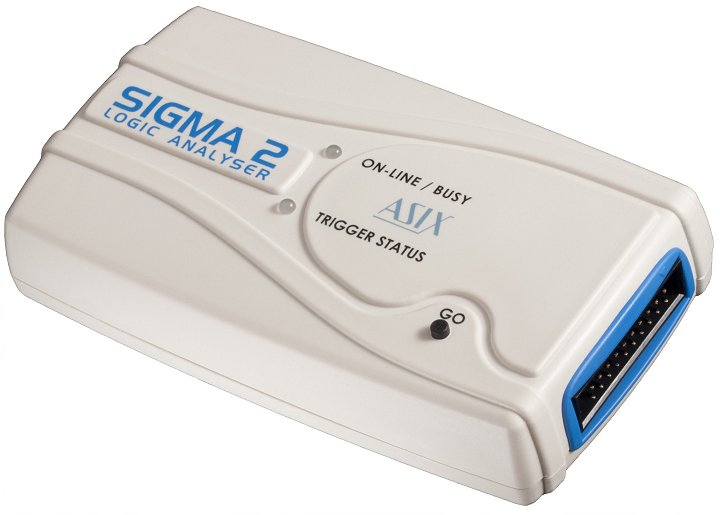
\includegraphics[width=5cm]{sigma2_720x515.jpg}
\end{center}
\subsection{Electrical connections to the Explorer 16 board}
Connect the analyser to the extension board with the numbered ribbon cable following this scheme:
\begin{center}
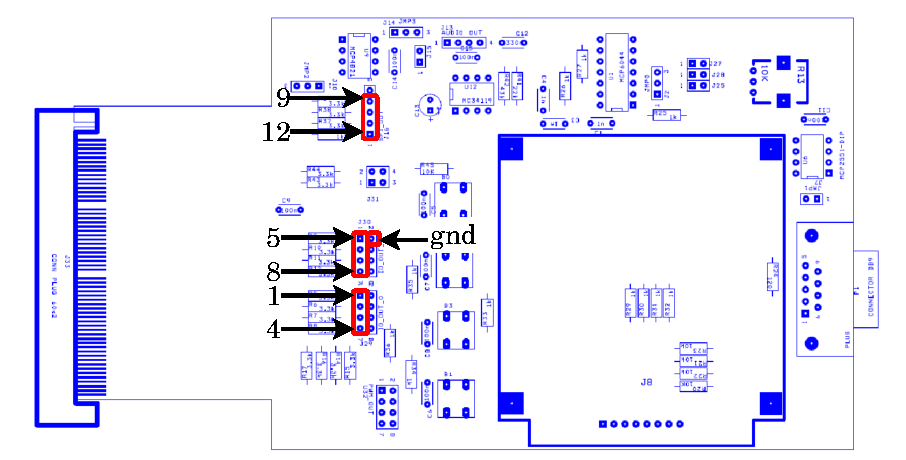
\includegraphics[width=11cm]{elec_con-crop.pdf}
\end{center}
\subsection{Software on the computer}

The software interface of the logic analyser looks like:

\begin{center}
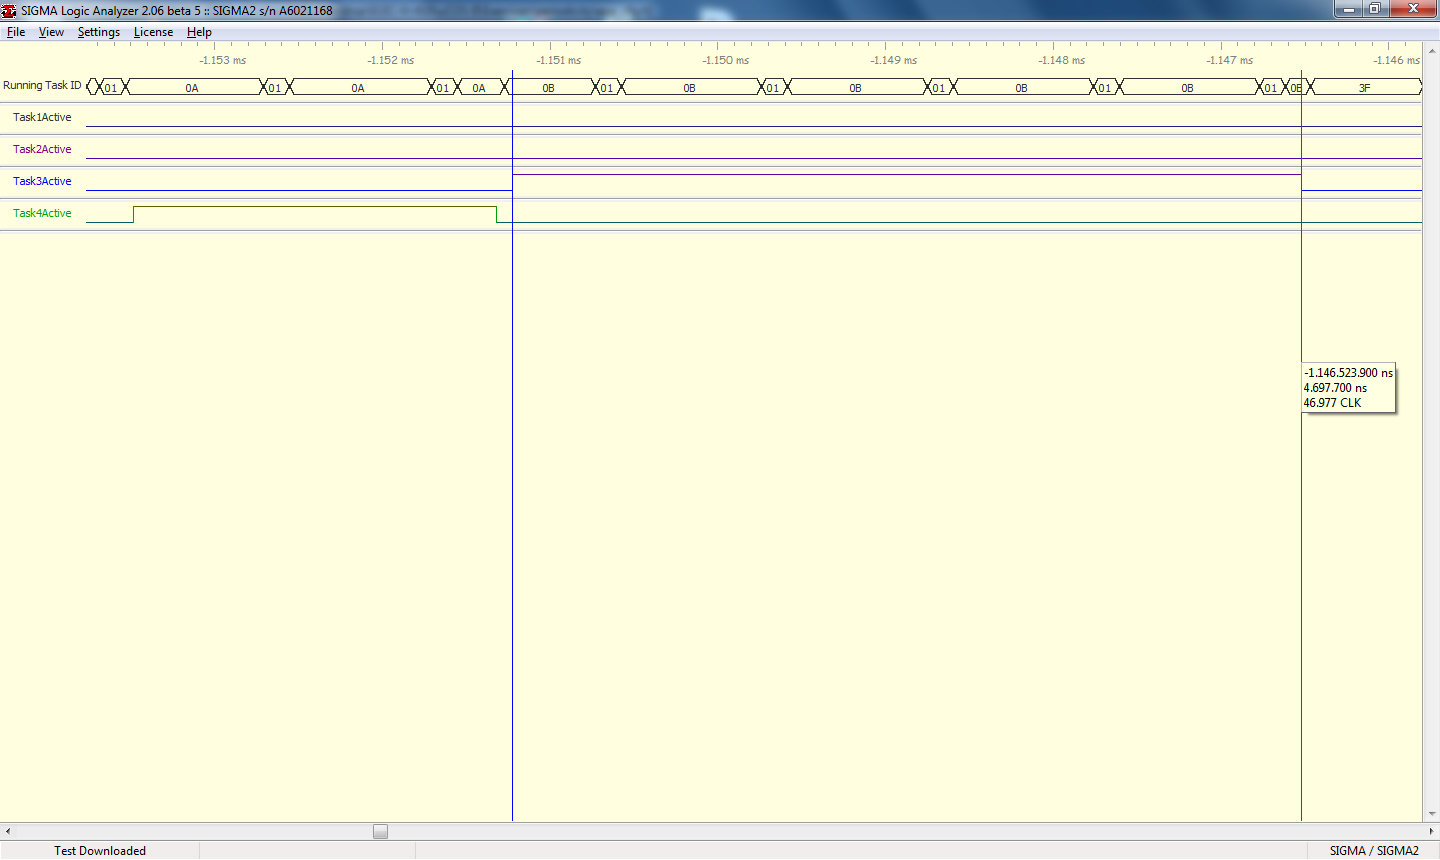
\includegraphics[width=16cm,trim= 0 100mm 0 0,clip]{Print_Screen_Logic_Analyzer.png}

\end{center}
\subsection{Basic measurements}
The red line on the screen is a cursor showing the time and values of signals in the main window. To place a marker (blue line), press space. If you move your cursor, the difference between the marker and the cursor will show in a tooltip.

The first acquisition must be launched by software. Following acquisitions can be done using the ``go" button of the analyser.
\end{document}
